\documentclass[paper=letter,11pt]{scrartcl}

\KOMAoptions{headinclude=true, footinclude=false}
\KOMAoptions{DIV=14, BCOR=5mm}
\KOMAoptions{numbers=noendperiod}
\KOMAoptions{parskip=half}
\addtokomafont{disposition}{\rmfamily}
\addtokomafont{part}{\LARGE}
\addtokomafont{descriptionlabel}{\rmfamily}
%\setkomafont{pageheadfoot}{\normalsize\sffamily}
\setkomafont{pagehead}{\normalsize\rmfamily}
%\setkomafont{publishers}{\normalsize\rmfamily}
\setkomafont{caption}{\normalfont\small}
\setcapindent{0pt}
\deffootnote[1em]{1em}{1em}{\textsuperscript{\thefootnotemark}\ }


\usepackage{amsmath}
\usepackage[varg]{txfonts}
\usepackage[T1]{fontenc}
\usepackage{graphicx}
\usepackage{xcolor}
\usepackage[american]{babel}
% hyperref is needed in many places, so include it here
\usepackage{hyperref}

\usepackage{xspace}
\usepackage{multirow}
\usepackage{float}


\usepackage{braket}
\usepackage{bbm}
\usepackage{relsize}
\usepackage{tcolorbox}


\def\x{\ensuremath{x}}
\def\xp{\ensuremath{x'}}
\def\t{\ensuremath{t}}
\def\tp{\ensuremath{t'}}
\def\v{\ensuremath{v}}
%\def\nus{$\nu$s}

%\def\ketY{\ensuremath{\ket {\Psi}}}
%\def\iGeV{\ensuremath{\textrm{GeV}^{-1}}}
%%\def\mp{\ensuremath{m_{\textrm{proton}}}}
%\def\rp{\ensuremath{r_{\textrm{proton}}}}
%\def\me{\ensuremath{m_{\textrm{electron}}}}
%\def\aG{\ensuremath{\alpha_G}}
%\def\rAtom{\ensuremath{r_{\textrm{atom}}}}
%\def\rNucl{\ensuremath{r_{\textrm{nucleus}}}}
%\def\GN{\ensuremath{\textrm{G}_\textrm{N}}}
%\def\ketX{\ensuremath{\ket{\vec{x}}}}
%\def\ve{\ensuremath{\vec{\epsilon}}}
%
%
%\def\ABCDMatrix{\ensuremath{\begin{pmatrix} A &  B  \\ C  & D \end{pmatrix}}}
%\def\xyprime{\ensuremath{\begin{pmatrix} x' \\ y' \end{pmatrix}}}
%\def\xyprimeT{\ensuremath{\begin{pmatrix} x' &  y' \end{pmatrix}}}
%\def\xy{\ensuremath{\begin{pmatrix} x \\ y \end{pmatrix}}}
%\def\xyT{\ensuremath{\begin{pmatrix} x & y \end{pmatrix}}}
%
%\def\IMatrix{\ensuremath{\begin{pmatrix} 0 &  1  \\ -1  & 0 \end{pmatrix}}}
%\def\IBoostMatrix{\ensuremath{\begin{pmatrix} 0 &  1  \\ 1  & 0 \end{pmatrix}}}
%\def\JThree{\ensuremath{\begin{pmatrix}    0 & -i & 0  \\ i & 0  & 0 \\ 0 & 0 & 0 \end{pmatrix}}} 
%\def\JTwo{\ensuremath{\begin{bmatrix}    0 & 0 & -i  \\ 0 & 0  & 0 \\ i & 0 & 0 \end{bmatrix}}}
%\def\JOne{\ensuremath{\begin{bmatrix}    0 & 0 & 0  \\ 0 & 0  & -i \\ 0 & i & 0 \end{bmatrix}}}
%\def\etamn{\ensuremath{\eta_{\mu\nu}}}
%\def\Lmn{\ensuremath{\Lambda^\mu_\nu}}
%\def\dmn{\ensuremath{\delta^\mu_\nu}}
%\def\wmn{\ensuremath{\omega^\mu_\nu}}
%\def\be{\begin{equation*}}
%\def\ee{\end{equation*}}
%\def\bea{\begin{eqnarray*}}
%\def\eea{\end{eqnarray*}}
%\def\bi{\begin{itemize}}
%\def\ei{\end{itemize}}
%\def\fmn{\ensuremath{F_{\mu\nu}}}
%\def\fMN{\ensuremath{F^{\mu\nu}}}
%\def\bc{\begin{center}}
%\def\ec{\end{center}}
%\def\nus{$\nu$s}

\def\adagger{\ensuremath{a_{p\sigma}^\dagger}}
\def\lineacross{\noindent\rule{\textwidth}{1pt}}

\newcommand{\multiline}[1] {
\begin{tabular} {|l}
#1
\end{tabular}
}

\newcommand{\multilineNoLine}[1] {
\begin{tabular} {l}
#1
\end{tabular}
}



\newcommand{\lineTwo}[2] {
\begin{tabular} {|l}
#1 \\
#2
\end{tabular}
}

\newcommand{\rmt}[1] {
\textrm{#1}
}


%
% Units
%
\def\m{\ensuremath{\rmt{m}}}
\def\GeV{\ensuremath{\rmt{GeV}}}
\def\pt{\ensuremath{p_\rmt{T}}}


\def\parity{\ensuremath{\mathcal{P}}}

\usepackage{cancel}
\usepackage{ mathrsfs }
\def\bigL{\ensuremath{\mathscr{L}}}

\usepackage{ dsfont }

\def\nus{$\nu$s}
\def\nue{\ensuremath{\nu_e}}
\def\numu{\ensuremath{\nu_\mu}}
\def\nutau{\ensuremath{\nu_\tau}}
\def\nualpha{\ensuremath{\nu_\alpha}}
\def\nuone{\ensuremath{\nu_1}}
\def\nutwo{\ensuremath{\nu_2}}
\def\nuthree{\ensuremath{\nu_3}}


\usepackage{fancyhdr}
\fancyhf{}



\lhead{\Large 33-211} % \hfill Introduction to Particle Physics \hfill Spring 2022}
\chead{\Large Physics 3 : Modern Essentials} % \hfill Spring 2022}
\rhead{\Large Spring 2025} % \hfill Introduction to Particle Physics \hfill Spring 2022}
\begin{document}
\thispagestyle{fancy}





%\begin{tabular}{c}
%{\large 33-444 \hfill Intro To Particle \hfill Spring 2019\\}
%\hline 
%\end{tabular}

\begin{center}
{\huge \textbf{Exam \#1}}
\large

\end{center}

{\large


\textbf{1) Cosmic Speedometer }\hfill \textit{(4 points)}\\
If you see a person traveling through space at half the speed of light, you will also see his clocks running:

\begin{itemize}
\item[a)] at half their normal speed
\item[b)] slower than half their normal speed
\item[c)] slower, but not slowed to half speed
\item[d)] at normal speed
\item[e)] backwards
\end{itemize}

\vspace{0.1in}

\textbf{2) High-speed spear }\hfill \textit{(4 points)}\\
A spear 10m long is thrown at a relativistic speed through a pipe that is 10 m long.
Both these dimensions are measured when each is at rest.
When the spear passes through the pipe, which of the following statements best describes what is observed?
\begin{itemize}
\item[a)] The spear shrinks so that the pipe completely covers it as some point
\item[b)] the pipe shrinks so that the spear extends from both ends at some point
\item[c)] both shrink equally so the pipe just covers the spear at some point
\item[d)] any of these, depending on the motion of the observer
\end{itemize}

\vspace{0.1in}

\textbf{3) Invariants }\hfill \textit{(8 points)}\\
Which of the following are invariant (ie: agreed on by all inertial observers)?
\begin{itemize}
\item[a)] time ordering of time-like separated events
\item[c)] component of the velocity of a projectile parallel to relative direction of motion
\item[b)] component of the velocity of a projectile perpendicular to relative direction of motion
\item[c)] time between events
\item[d)] distance between events
\item[e)] total particle speed when beta < 1
\item[f)] total particle speed when beta = 1
\item[g)] proper time along a world line
\end{itemize}

\clearpage

\textbf{4) Relative velocities }\hfill \textit{(12 points)}\\

A rocket ship moving at 0.5c wrt earth fires a missile which moves at 0.8c wrt the rocket.
What is the speed of the missile wrt earth, assuming classical physics (Galilean transformations)?
What is the speed of the missile wrt earth, assuming relativity (Lorentz transformations)?

\vspace{2.8in}

\textbf{5) Causality}  \hfill \textit{(12 points)}\\
You are located at the origin of the S frame: (x,t)=(0,0).
Your friend is located at the origin of the S` which is moving to the right at $\beta = 0.99$ wrt the S frame in the usual way with origins coinciding at (0,0).
Consider the following space-time events (coordinates in S):\\
\begin{tabular}{clr}
  & (x,& t)\\
  \hline
  A = & (0   , & 2)\\
  B = & (2.01, & 2)\\
  C = & (1.99, & 2)\\
  D = & (2,    & 0)\\
  E = & (0,    & -2)\\
  F = & (2,    & -1.99)\\
  G = & (2,    & -2.01)\\
\end{tabular}

\vspace{0.1in}

a) Which events can you causally effect ?\\

b) Which events can your friend causally effect ?\\

c) Which events can casually effect you?\\

d) Which events can casually effected your friend?

%a) Argue with a space diagram that casualty (ie: time-ordering) is preserved 
%is causes propogate at beta < 0. 
%
%\vspace{2in}
%b) Argue with a space diagram that casality (ie: time-ordering) is NOT preserved 
%if beta > 1
%\vspace{2in}
\clearpage

\textbf{6) Olsen twins}  \hfill \textit{(15 points)}\\
Mary-Kate and Ashley are famous child twin actors.
They decide to try to prolong their combined effective career by sending one of them on a high-speed round-trip journey. 
Mary-Kay travels at speed $\beta = 24/25$ away from earth for 7 years as measured by her.
She then turns around and returns to earth with speed $\beta = 24/25$.

a) How much older is Mary-Kate when she returns ?

b) How much older is Ashley when Mary-Kate returns ?


\clearpage


\textbf{7) Analyze the Michelson and Morely experiment in \underline{the fixed star frame}.}  \hfill \textit{(20 points)}\\
Show that the null effect  ($\Delta t = 0$) can be accounted for with Relativity.

\clearpage
\textbf{8) Space-time diagrams}  \hfill \textit{(15 points)}\\
Frames S and S' are moving relative to each other along the x axis.
In frame S, Event A occurs at $x_A = 0.5 m$ and $t_A = 0.5 m$ and Event B occurs at $x_B = -2.0 m$ and $t_B = -0.5 m$.
The events are simultaneous in the S' frame.
\begin{itemize}
\item[a)] Mark the location of these events in the diagram below
\item[b)] Draw axis for the S' frame
\item[c)] From the diagram estimate $\beta$,  the magnitude and direction of the speed of S' relative to S.
\item[d)] Show where the two events occur in S'. \\(ie: mark the on the x' and t' axis the projected coordinates of A and B).
\end{itemize}
\vspace*{0.1in}

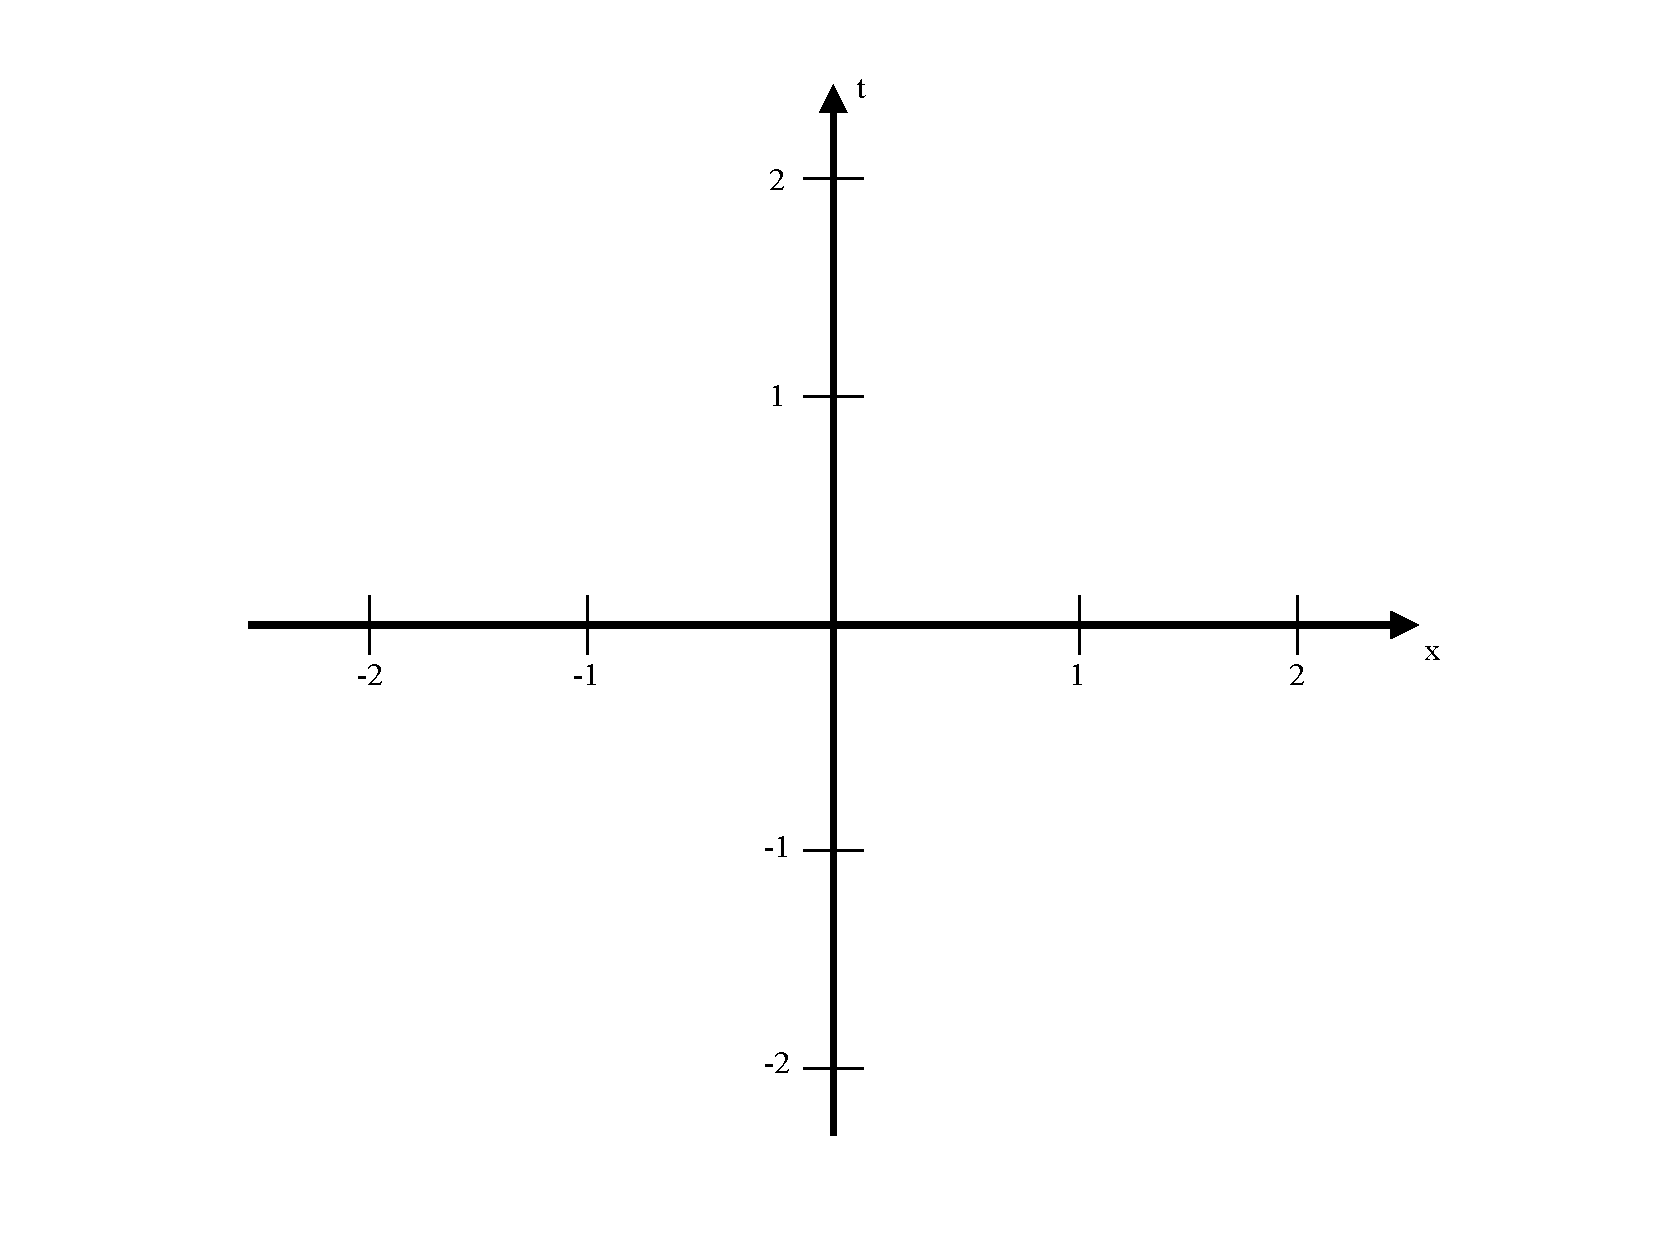
\includegraphics[width=1\textwidth]{./AxesCropped.pdf}



} % Begning Large
\end{document}
